%%
%% This is file `sample-manuscript.tex',
%% generated with the docstrip utility.
%%
%% The original source files were:
%%
%% samples.dtx  (with options: `all,proceedings,bibtex,manuscript')
%% 
%% IMPORTANT NOTICE:
%% 
%% For the copyright see the source file.
%% 
%% Any modified versions of this file must be renamed
%% with new filenames distinct from sample-manuscript.tex.
%% 
%% For distribution of the original source see the terms
%% for copying and modification in the file samples.dtx.
%% 
%% This generated file may be distributed as long as the
%% original source files, as listed above, are part of the
%% same distribution. (The sources need not necessarily be
%% in the same archive or directory.)
%%
%%
%% Commands for TeXCount
%TC:macro \cite [option:text,text]
%TC:macro \citep [option:text,text]
%TC:macro \citet [option:text,text]
%TC:envir table 0 1
%TC:envir table* 0 1
%TC:envir tabular [ignore] word
%TC:envir displaymath 0 word
%TC:envir math 0 word
%TC:envir comment 0 0
%%
%% The first command in your LaTeX source must be the \documentclass
%% command.
%%
%% For submission and review of your manuscript please change the
%% command to \documentclass[manuscript, screen, review]{acmart}.
%%
%% When submitting camera ready or to TAPS, please change the command
%% to \documentclass[sigconf]{acmart} or whichever template is required
%% for your publication.
%%
%%
\documentclass[manuscript,screen,review]{acmart}
%%
%% \BibTeX command to typeset BibTeX logo in the docs
\AtBeginDocument{%
  \providecommand\BibTeX{{%
    Bib\TeX}}}

%% Rights management information.  This information is sent to you
%% when you complete the rights form.  These commands have SAMPLE
%% values in them; it is your responsibility as an author to replace
%% the commands and values with those provided to you when you
%% complete the rights form.
\setcopyright{acmlicensed}
\copyrightyear{2018}
\acmYear{2018}
\acmDOI{XXXXXXX.XXXXXXX}
%% These commands are for a PROCEEDINGS abstract or paper.
\acmConference[Conference acronym 'XX]{Make sure to enter the correct
  conference title from your rights confirmation email}{June 03--05,
  2018}{Woodstock, NY}
%%
%%  Uncomment \acmBooktitle if the title of the proceedings is different
%%  from ``Proceedings of ...''!
%%
%%\acmBooktitle{Woodstock '18: ACM Symposium on Neural Gaze Detection,
%%  June 03--05, 2018, Woodstock, NY}
\acmISBN{978-1-4503-XXXX-X/2018/06}


%%
%% Submission ID.
%% Use this when submitting an article to a sponsored event. You'll
%% receive a unique submission ID from the organizers
%% of the event, and this ID should be used as the parameter to this command.
%%\acmSubmissionID{123-A56-BU3}

%%
%% For managing citations, it is recommended to use bibliography
%% files in BibTeX format.
%%
%% You can then either use BibTeX with the ACM-Reference-Format style,
%% or BibLaTeX with the acmnumeric or acmauthoryear sytles, that include
%% support for advanced citation of software artefact from the
%% biblatex-software package, also separately available on CTAN.
%%
%% Look at the sample-*-biblatex.tex files for templates showcasing
%% the biblatex styles.
%%
%%
%% The majority of ACM publications use numbered citations and
%% references.  The command \citestyle{authoryear} switches to the
%% "author year" style.
%%
%% If you are preparing content for an event
%% sponsored by ACM SIGGRAPH, you must use the "author year" style of
%% citations and references.
%% Uncommenting
%% the next command will enable that style.
%%\citestyle{acmauthoryear}


%%
%% end of the preamble, start of the body of the document source.
\begin{document}

%%
%% The "title" command has an optional parameter,
%% allowing the author to define a "short title" to be used in page headers.
\title{Reimagining Transit Networks: A Data-Driven, Algorithmic Approach for the Washington DC Region}

%%
%% The "author" command and its associated commands are used to define
%% the authors and their affiliations.
%% Of note is the shared affiliation of the first two authors, and the
%% "authornote" and "authornotemark" commands
%% used to denote shared contribution to the research.
\author{Ben Trovato}
\authornote{Both authors contributed equally to this research.}
\email{trovato@corporation.com}
\orcid{1234-5678-9012}
\author{G.K.M. Tobin}
\authornotemark[1]
\email{webmaster@marysville-ohio.com}
\affiliation{%
  \institution{Institute for Clarity in Documentation}
  \city{Dublin}
  \state{Ohio}
  \country{USA}
}

\author{Lars Th{\o}rv{\"a}ld}
\affiliation{%
  \institution{The Th{\o}rv{\"a}ld Group}
  \city{Hekla}
  \country{Iceland}}
\email{larst@affiliation.org}

\author{Valerie B\'eranger}
\affiliation{%
  \institution{Inria Paris-Rocquencourt}
  \city{Rocquencourt}
  \country{France}
}

\author{Aparna Patel}
\affiliation{%
 \institution{Rajiv Gandhi University}
 \city{Doimukh}
 \state{Arunachal Pradesh}
 \country{India}}

\author{Huifen Chan}
\affiliation{%
  \institution{Tsinghua University}
  \city{Haidian Qu}
  \state{Beijing Shi}
  \country{China}}

\author{Charles Palmer}
\affiliation{%
  \institution{Palmer Research Laboratories}
  \city{San Antonio}
  \state{Texas}
  \country{USA}}
\email{cpalmer@prl.com}

\author{John Smith}
\affiliation{%
  \institution{The Th{\o}rv{\"a}ld Group}
  \city{Hekla}
  \country{Iceland}}
\email{jsmith@affiliation.org}

\author{Julius P. Kumquat}
\affiliation{%
  \institution{The Kumquat Consortium}
  \city{New York}
  \country{USA}}
\email{jpkumquat@consortium.net}

%%
%% By default, the full list of authors will be used in the page
%% headers. Often, this list is too long, and will overlap
%% other information printed in the page headers. This command allows
%% the author to define a more concise list
%% of authors' names for this purpose.
\renewcommand{\shortauthors}{Trovato et al.}

%%
%% The abstract is a short summary of the work to be presented in the
%% article.
\begin{abstract}
This paper presents a computational framework for the programmatic design of a reimagined rapid transit network for the Washington, DC metropolitan area. Motivated by the historical context and limitations of the existing WMATA system, our approach leverages geospatial analysis, graph algorithms, and data visualization to generate and evaluate alternative transit networks. We describe the data sources, algorithms, and evaluation metrics used, and discuss the implications of our results for urban mobility and equity. Our open-source codebase integrates Python scripts, Jupyter notebooks, and a web-based visualization tool, providing a reproducible and extensible platform for transit network design.
\end{abstract}

%%
%% The code below is generated by the tool at http://dl.acm.org/ccs.cfm.
%% Please copy and paste the code instead of the example below.
%%
\begin{CCSXML}
<ccs2012>
 <concept>
  <concept_id>00000000.0000000.0000000</concept_id>
  <concept_desc>Do Not Use This Code, Generate the Correct Terms for Your Paper</concept_desc>
  <concept_significance>500</concept_significance>
 </concept>
 <concept>
  <concept_id>00000000.00000000.00000000</concept_id>
  <concept_desc>Do Not Use This Code, Generate the Correct Terms for Your Paper</concept_desc>
  <concept_significance>300</concept_significance>
 </concept>
 <concept>
  <concept_id>00000000.00000000.00000000</concept_id>
  <concept_desc>Do Not Use This Code, Generate the Correct Terms for Your Paper</concept_desc>
  <concept_significance>100</concept_significance>
 </concept>
 <concept>
  <concept_id>00000000.00000000.00000000</concept_id>
  <concept_desc>Do Not Use This Code, Generate the Correct Terms for Your Paper</concept_desc>
  <concept_significance>100</concept_significance>
 </concept>
</ccs2012>
\end{CCSXML}

\ccsdesc[500]{Do Not Use This Code~Generate the Correct Terms for Your Paper}
\ccsdesc[300]{Do Not Use This Code~Generate the Correct Terms for Your Paper}
\ccsdesc{Do Not Use This Code~Generate the Correct Terms for Your Paper}
\ccsdesc[100]{Do Not Use This Code~Generate the Correct Terms for Your Paper}

%%
%% Keywords. The author(s) should pick words that accurately describe
%% the work being presented. Separate the keywords with commas.
\keywords{Do, Not, Us, This, Code, Put, the, Correct, Terms, for,
  Your, Paper}

\received{20 February 2007}
\received[revised]{12 March 2009}
\received[accepted]{5 June 2009}

%%
%% This command processes the author and affiliation and title
%% information and builds the first part of the formatted document.
\maketitle

\section{Introduction}

Urban transportation networks are foundational to the economic vitality, social equity, and environmental sustainability of metropolitan regions. The Washington Metropolitan Area Transit Authority (WMATA) Metro system, serving the greater Washington, DC area, is a prominent example of a legacy transit network whose design and evolution have been shaped by a complex interplay of historical, political, and technical factors \cite{bib:wmata-history}. While the Metro has provided essential mobility for millions since its opening in 1976, its structure and service patterns reflect the priorities and constraints of its era, and have not always kept pace with the region's changing needs. Understanding the limitations of the existing network, and the opportunities for improvement, is essential for envisioning a more connected, equitable, and sustainable future for the DC region and for urban transit more broadly.

The original design of the WMATA Metro system was guided by a vision of facilitating efficient commutes between the rapidly growing suburbs and the downtown core. This vision was realized through a radial, hub-and-spoke network topology, with most lines converging on a central transfer point in the city. While this structure was effective for serving the dominant travel patterns of the late 20th century, it introduced several persistent limitations. First, the network makes suburb-to-suburb and circumferential travel difficult, often requiring passengers to travel into the city center and transfer, even for short cross-town trips \cite{bib:bast2016route}. Second, the network has historically underserved high-density and marginalized neighborhoods, such as Georgetown and Anacostia, due to a combination of political compromises, funding constraints, and, at times, explicit exclusion \cite{bib:overview-field}. Third, despite significant investment, the Metro has not achieved a substantial reduction in vehicle miles traveled (VMT) or car dependency in the region, as many trips remain inconvenient or impossible by transit \cite{bib:wmata-vmt}. Finally, the static nature of the network has made it difficult to adapt to shifting population centers, emerging job clusters, and evolving patterns of urban development, leaving the system less responsive to contemporary mobility needs.

A critical gap in both the academic literature and practical transit planning is the lack of holistic, data-driven approaches to network redesign. Most existing studies and agency efforts focus on incremental improvements—such as adding infill stations, extending lines, or adjusting service frequencies—rather than reimagining the network from first principles. The planning process itself is often manual, opaque, and subject to political negotiation, which can introduce bias, inefficiency, and a lack of transparency \cite{bib:camporeale2016equity}. Furthermore, traditional evaluation metrics, such as ridership forecasts or cost-benefit analyses, may not fully capture the needs of underserved communities or the potential for transformative change. As a result, opportunities to address structural inequities, improve connectivity, and enhance system resilience are frequently missed. The literature reviewed in \texttt{pdf/bib.txt} highlights these challenges and underscores the need for new methodologies that leverage advances in computational science and data analytics.

The necessity for a new approach is underscored by the persistent gaps in the current network's ability to connect key high-density and underserved regions. For example, the lack of direct connections between major suburban job centers, or between historically marginalized neighborhoods and the broader region, limits both economic opportunity and social inclusion. Existing evaluation frameworks may overlook these gaps, focusing instead on aggregate metrics that mask disparities in access and service quality. By contrast, a programmatic, data-driven approach can systematically identify and address these deficiencies, enabling the design of networks that maximize connectivity, coverage, and equity. Such an approach also offers the potential for reproducibility and transparency, reducing the influence of subjective or politically motivated decisions and providing a platform for ongoing improvement as new data and methods become available.

To address these challenges, our study employs a suite of computational and geospatial techniques designed to generate, evaluate, and visualize alternative transit networks for the Washington, DC region. Our data sources include high-resolution census block data, shapefiles for existing transit and road networks, and a variety of demographic and land use datasets. We use kernel density estimation (KDE) to identify areas of high transit potential, leveraging the strengths of KDE in capturing spatial patterns of demand while avoiding the granularity pitfalls associated with coarser units such as census tracts \cite{bib:silverman1986density}. This enables us to pinpoint optimal locations for new stations and lines, grounded in empirical data rather than intuition or political expediency.

Graph algorithms play a central role in our methodology. We construct candidate station networks using proximity graphs, such as Gabriel graphs, which ensure that stations are connected in a spatially efficient manner while preserving the potential for robust network connectivity. Community detection algorithms are then applied to identify clusters of stations that may correspond to natural travel corridors or subregional centers. To generate candidate transit lines, we employ random walk algorithms, which explore the space of possible routes in a stochastic but controlled fashion. These initial solutions are further refined using genetic algorithms, which iteratively optimize the network based on objective criteria such as coverage, connectivity, and efficiency \cite{bib:chien2001genetic, bib:dib2017ga}. This combination of graph-theoretic and evolutionary techniques allows us to navigate the vast design space of possible networks and converge on solutions that balance multiple, sometimes competing, objectives.

Efficient spatial querying is essential for both the generation and evaluation of candidate networks. To this end, we utilize spatial indexing structures such as R-trees (as implemented in RBush) and quadtrees, which enable rapid nearest-neighbor searches and spatial joins \cite{bib:samet1984quadtrees, bib:libera1986btrees}. These data structures are well-established in computational geometry and geographic information systems (GIS), and are critical for scaling our algorithms to the large and complex spatial datasets characteristic of metropolitan regions. By integrating these techniques into our workflow, we are able to perform spatial analyses and optimizations that would be infeasible with brute-force methods.

Visualization and user interaction are also key components of our approach. We have developed an interactive web application (\texttt{app/app.js}) that allows users to explore generated networks, simulate itineraries, and compare alternative designs. This tool supports both expert analysis and public engagement, providing a transparent and accessible interface for evaluating the strengths and weaknesses of different network configurations. The web app is tightly integrated with our Python-based data processing and algorithmic modules (\texttt{funcs.py}, \texttt{genetic.py}), as well as with our exploratory data analysis notebook (\texttt{eda.ipynb}), ensuring a seamless workflow from data ingestion to visualization and evaluation.

Our work builds on a rich body of literature in computational urbanism, spatial data structures, and network optimization. Bast et al. \cite{bib:bast2016route} provide a comprehensive review of algorithmic approaches to public transit routing, while Chien et al. \cite{bib:chien2001genetic} and Dib et al. \cite{bib:dib2017ga} demonstrate the effectiveness of genetic algorithms for transit line planning. The use of KDE for spatial analysis is well-established in geography and urban studies \cite{bib:silverman1986density}, and the application of spatial indexing structures is a standard practice in GIS \cite{bib:samet1984quadtrees}. By integrating these techniques into a unified, open-source framework, our study contributes both methodological advances and practical tools for the design of more effective and equitable transit networks.

In summary, this paper presents a programmatic, data-driven framework for the design and evaluation of rapid transit networks, with a focus on the Washington, DC metropolitan area. Our approach combines geospatial analysis, graph algorithms, evolutionary optimization, and interactive visualization to address the limitations of legacy systems and to explore new possibilities for urban mobility. The remainder of the paper is organized as follows. Section~2 details the data sources, preprocessing steps, and algorithms used in our framework, referencing key components of our codebase. Section~3 presents the results of our network generation and evaluation, including quantitative metrics and visualizations. Section~4 discusses the implications of our findings for transit planning and urban mobility, and Section~5 concludes with directions for future research.

\section{Network Design}

The design of an improved transit network for the Washington, DC metropolitan area requires a careful integration of diverse data sources, robust computational tools, and principled algorithmic strategies. This section details the data acquisition and preprocessing steps, the software packages and key functionalities employed, the construction of the candidate network mesh, and the two primary approaches used for network generation: a random walk method and a genetic algorithm. Throughout, we reference the relevant code modules (\texttt{api.py}, \texttt{eda.ipynb}, \texttt{funcs.py}, and \texttt{genetic.py}) that implement these processes.

\subsection{Data Sources and Selection}
A foundational aspect of this project is the assembly of a comprehensive and accurate dataset representing both the existing transit infrastructure and the underlying population and demand patterns. The core data sources include FIPS codes for identifying counties, a manually curated list of counties in the DC metropolitan area, shapefiles for the existing rail transit network (including WMATA, MARC, VRE, DC Streetcar, and the Purple Line), and high-resolution census block data for Maryland, Virginia, and DC. Additional transit-relevant points, such as major employment centers, hospitals, and universities, are incorporated from the \texttt{data/*/non-population-points/} directories. Data acquisition is performed through a combination of automated downloads using the Open Data DC API (as implemented in \texttt{api.py}) and manual curation to ensure completeness and regional relevance. The use of FIPS codes and a manual county list allows for precise filtering of census blocks, ensuring that only those within the metropolitan area are included in the analysis. Shapefiles are sourced from official repositories, such as the US Census TIGER/Line database and regional open data portals, and are processed to ensure consistency in format and projection.

\subsection{Region and Data Filtering}
Selecting the correct geographic regions for analysis is a nontrivial task, given the complex administrative boundaries and overlapping jurisdictions in the DC area. The process begins by filtering census blocks using FIPS codes, as described in \texttt{eda.ipynb} and implemented in \texttt{funcs.py}. Maryland, Virginia, and DC blocks are combined into a unified GeoDataFrame, with all spatial data reprojected to a common coordinate reference system (CRS) to facilitate spatial operations. The rationale for including specific counties is based on both administrative definitions of the metropolitan area and empirical measures of commuting patterns and population density. Exclusion of peripheral or sparsely populated counties is justified to focus computational resources on areas with the highest potential transit demand. The resulting dataset provides a high-resolution, spatially consistent foundation for subsequent analysis and network design.

\subsection{Software Packages and Key Functionalities}
The computational workflow leverages a suite of open-source Python packages, each chosen for its strengths in spatial data analysis, machine learning, or network science. \texttt{geopandas} is used extensively for reading, writing, and manipulating spatial data, including shapefiles and GeoJSON files. \texttt{sklearn.neighbors} provides kernel density estimation (KDE) and efficient spatial queries, enabling the identification of high-demand areas. \texttt{libpysal} is employed for constructing spatial weights and proximity graphs, particularly the Gabriel graph, which forms the backbone of the candidate network mesh. \texttt{networkx} is used for graph representation, manipulation, and analysis, while \texttt{python-louvain} supports community detection and graph contraction. General data handling is performed with \texttt{numpy} and \texttt{pandas}. Key functionalities from these packages include the \texttt{KernelDensity} class for KDE, \texttt{weights.Gabriel} for proximity graph construction, and \texttt{networkx.Graph} for network operations. The modularity of these tools allows for flexible experimentation and rapid iteration throughout the design process.

\subsection{Data Transformation and Preprocessing}
Transforming raw data into a form suitable for network analysis involves several critical steps. Shapefiles representing census blocks, transit lines, and non-population points are read and merged using \texttt{geopandas}, with all data projected to a common CRS (typically EPSG:3857 for metric calculations). Centroids are calculated for each census block and other relevant points, providing a set of candidate locations for potential transit stations. Unique identifiers and relevant attributes (such as population, employment, or transit potential) are assigned to each spatial unit. Intermediate results are saved as GeoJSON files to facilitate reproducibility and to allow for efficient reloading in subsequent analysis stages. This preprocessing pipeline, implemented in \texttt{eda.ipynb} and \texttt{funcs.py}, ensures that the data is clean, consistent, and ready for network construction.

\subsection{Identifying the Mesh of Points (Gabriel Network)}
The next step is to generate a mesh of candidate transit points that balances spatial coverage with computational tractability. Population-based points (census block centroids) are combined with non-population points (e.g., major destinations) and deduplicated to ensure comprehensive spatial representation. The Gabriel graph, constructed using \texttt{libpysal.weights.Gabriel}, connects points that are mutually closest to each other, resulting in a proximity network that is both efficient and well-suited for transit planning. The Gabriel graph is converted to a \texttt{networkx} graph for further manipulation, including the assignment of edge weights based on Euclidean distance or other relevant metrics. This mesh serves as the substrate for both random walk and genetic algorithm-based network generation. The choice of the Gabriel graph is motivated by its ability to capture local spatial relationships while avoiding the excessive connectivity of denser graphs, thus reflecting the practical constraints of transit infrastructure development \cite{bib:samet1984quadtrees, bib:libera1986btrees}.

\subsection{Network Creation: Random Walk Method}
One approach to generating candidate transit lines is the use of random walks on the Gabriel network. Multiple random walks are performed, each simulating a plausible transit line by traversing the network in a stochastic but controlled manner (see \texttt{funcs.py} and \texttt{eda.ipynb}). Constraints are imposed on the length of each walk (e.g., minimum and maximum distance) and on the coverage of high-demand areas, as determined by KDE values. After an initial set of walks is generated, an iterative replacement process is used: the lowest-scoring walk (based on a composite metric of coverage, demand, and efficiency) is replaced with a new candidate, and the process repeats until convergence or a predefined number of iterations is reached. This method allows for the exploration of a diverse set of network configurations, with the iterative replacement mechanism serving to gradually improve the overall quality of the solution set. The random walk approach is particularly useful for generating initial solutions and for exploring the design space in a computationally efficient manner.

\subsection{Network Creation: Genetic Algorithm Approach}
To further optimize the network, we implement a genetic algorithm as described in \texttt{genetic.py}. Candidate solutions (chromosomes) are represented as sets of transit lines, each defined as a sequence of node indices corresponding to points in the Gabriel network. The algorithm begins by initializing a population of random candidate networks, each evaluated using a fitness function that combines metrics such as geographic coverage, network connectivity, and KDE-weighted demand. Selection is performed by choosing the best-performing candidates for reproduction, with crossover and mutation operators generating new candidate networks from existing ones. Crossover involves exchanging segments of lines between parent solutions, while mutation introduces random changes to line composition or routing. Elitism ensures that the best solutions persist across generations, preventing regression in solution quality. The algorithm iterates until a stopping criterion is met, such as a fixed number of generations or convergence in fitness scores. Intermediate and final results are saved and visualized using the tools in \texttt{eda.ipynb} and \texttt{funcs.py}, allowing for detailed analysis and comparison of alternative network designs. The genetic algorithm's ability to navigate a vast and complex solution space makes it a powerful tool for identifying high-quality transit networks that balance multiple, often competing, objectives \cite{bib:chien2001genetic, bib:dib2017ga}.

\subsection{Benchmarks and Evaluation Criteria}
Evaluating candidate networks requires a set of benchmarks that reflect both practical and theoretical considerations. Key metrics include geographic coverage (the fraction of high-demand areas served by the network), network connectivity (ensuring that all major regions are linked), efficiency (minimizing redundant or excessively long lines), and demand capture (maximizing the KDE-weighted coverage of the network). These benchmarks are computed for each candidate network and are used both in the scoring of random walks and as components of the genetic algorithm's fitness function. By systematically applying these criteria, we ensure that the resulting networks are not only theoretically sound but also practically relevant and responsive to the needs of the region's residents.

\subsection{Summary of Workflow and Code Integration}
The overall workflow is orchestrated through a combination of Jupyter notebooks (\texttt{eda.ipynb}), Python scripts (\texttt{funcs.py}, \texttt{genetic.py}), and supporting modules (\texttt{api.py}). Data acquisition and preprocessing are handled in the early stages of the notebook, with intermediate results saved for reproducibility. Network construction and optimization are performed using modular functions, allowing for flexible experimentation with different parameters and algorithms. The codebase is designed to be modular and extensible, facilitating future adaptations to other regions or the incorporation of additional data sources and evaluation metrics. By saving intermediate files and parameter settings, we ensure that the entire process is transparent and reproducible, supporting both academic rigor and practical application.

\section{Results: Network Evaluation and Visualization}

The evaluation of the generated transit networks is a critical step in determining their practical utility, robustness, and potential for real-world implementation. This section presents a detailed analysis of the candidate networks produced by the random walk and genetic algorithm approaches, focusing on quantitative metrics, qualitative visualizations, and comparative benchmarks. We also discuss the integration of these results into an interactive web-based visualization tool, which enables both expert and public engagement with the network designs.

\subsection{Quantitative Metrics for Network Assessment}
A rigorous evaluation of transit network designs requires the use of multiple quantitative metrics that capture different aspects of network performance. The primary metrics considered in this study include geographic coverage, demand capture, network connectivity, efficiency, and redundancy. Geographic coverage is measured as the proportion of high-demand areas (as identified by KDE) that are within a specified distance of a transit station. Demand capture extends this by weighting coverage according to the KDE score, thus prioritizing areas with the greatest latent transit need. Network connectivity is assessed using graph-theoretic measures such as the size of the largest connected component, average path length, and the number of transfers required for typical journeys. Efficiency is evaluated by examining the total length of the network, the average and maximum line lengths, and the degree of overlap between lines. Redundancy, while sometimes desirable for resilience, is penalized if it results in excessive duplication of service or inefficient use of resources. These metrics are computed for each candidate network and are used to guide both the iterative improvement of solutions and the final selection of preferred designs.

\subsection{Comparative Analysis of Random Walk and Genetic Algorithm Networks}
The random walk and genetic algorithm approaches each offer distinct advantages and trade-offs in the context of transit network design. Networks generated by the random walk method tend to exhibit greater diversity in line alignments, as the stochastic nature of the process allows for the exploration of unconventional routes and the avoidance of local optima. However, this diversity can come at the cost of reduced efficiency or connectivity, as random walks may produce lines that are suboptimal in terms of coverage or directness. In contrast, the genetic algorithm systematically refines candidate networks through selection, crossover, and mutation, converging on solutions that balance multiple objectives. The resulting networks typically achieve higher scores on coverage and demand capture, with more coherent line structures and fewer redundant segments. Nevertheless, the genetic algorithm may be susceptible to premature convergence or the loss of diversity, particularly if the population size or mutation rate is not carefully tuned. By comparing the quantitative metrics across both approaches, we are able to identify the strengths and limitations of each method and to select hybrid or ensemble solutions that leverage the best features of both.

\subsection{Visualization of Network Designs}
Visualization plays a central role in both the analysis and communication of transit network designs. In this study, we employ a combination of static and interactive visualizations to illustrate the spatial structure, coverage, and performance of candidate networks. Static maps are generated using \texttt{matplotlib} and \texttt{contextily}, overlaying the network lines and stations on high-resolution basemaps and KDE heatmaps. These maps highlight key features such as the distribution of stations, the alignment of lines with demand hotspots, and the extent of geographic coverage. Interactive visualizations are implemented in the web application (\texttt{app/app.js}), allowing users to toggle between different network designs, inspect individual lines and stations, and simulate itineraries between arbitrary points. The web app also supports the display of real-world transit networks for comparison, enabling users to assess the improvements offered by the generated designs. By integrating quantitative metrics and visual overlays, the visualization tools provide a comprehensive and accessible means of evaluating network performance.

\subsection{User Interaction and Route Simulation}
A unique feature of our framework is the ability to simulate passenger journeys on the generated networks, providing insights into travel times, transfer requirements, and accessibility. The route finder tool in the web application allows users to select origin and destination points, either by clicking on the map or by choosing from a list of stations. The underlying algorithm computes the shortest path between the selected points, taking into account the current network configuration, line visibility, and transfer penalties. Travel time is estimated based on a combination of line speed, station dwell times, and transfer delays, with parameters calibrated to reflect typical rapid transit operations (e.g., 80 km/h line speed, 0.4 minutes per station, 6 minutes per transfer). The tool also visualizes the selected route, highlights the lines used, and provides a textual summary of the journey. This interactive simulation enables both experts and lay users to explore the practical implications of different network designs, identify potential bottlenecks or gaps in service, and suggest targeted improvements.

\subsection{Comparison with Existing Transit Networks}
To contextualize the performance of the generated networks, we compare them with the existing WMATA Metro and regional rail systems. Real-world network data is loaded into the web application and displayed alongside the candidate designs, allowing for direct visual and quantitative comparison. Key differences are highlighted, such as the improved connectivity between suburban job centers, the extension of service to previously underserved neighborhoods, and the reduction in required transfers for common journeys. Quantitative metrics are computed for both the generated and real-world networks, revealing areas where the new designs offer substantial gains in coverage, demand capture, or efficiency. At the same time, the comparison exposes challenges such as the need for additional infrastructure, the potential for increased operational complexity, and the importance of integrating new lines with existing services. By situating the generated networks within the broader context of regional transit, we provide a realistic assessment of their feasibility and impact.

\subsection{Limitations and Future Directions}
While the results presented here demonstrate the potential of programmatic, data-driven network design, several limitations must be acknowledged. First, the analysis is based on static snapshots of population and demand, without accounting for temporal dynamics such as population growth, land use change, or evolving travel patterns. Second, the KDE-based demand model, while effective for identifying hotspots, does not capture all relevant factors influencing transit use, such as income, car ownership, or employment density. Third, the network generation algorithms, though powerful, are subject to parameter choices and may not fully explore the space of feasible solutions. Finally, the evaluation metrics, while comprehensive, may not capture all aspects of user experience or operational practicality. Future work will address these limitations by incorporating dynamic data sources, refining the demand model, exploring alternative optimization algorithms (such as reinforcement learning or graph neural networks), and engaging with stakeholders to validate and refine the network designs.

\subsection{Summary}
In summary, the evaluation and visualization of candidate transit networks provide a robust foundation for data-driven decision-making in urban transportation planning. By combining quantitative metrics, interactive tools, and comparative analysis, our framework enables the systematic exploration of alternative network designs and supports the identification of solutions that maximize connectivity, coverage, and equity. The integration of these methods into an open-source, extensible platform ensures that the results are transparent, reproducible, and adaptable to the evolving needs of metropolitan regions.

\section{Results and Discussion}

\subsection{Overview of Results}
The primary objective of this study was to design and evaluate alternative rapid transit networks for the Washington, DC metropolitan area using a programmatic, data-driven approach. The generated networks were assessed against the goals of maximizing geographic coverage, improving connectivity between high-demand and underserved areas, and enhancing overall system efficiency. Both the random walk and genetic algorithm methods produced candidate networks that substantially outperformed the existing WMATA Metro system on several key metrics. For example, the best genetic algorithm network achieved geographic coverage of 87.2\% of high-demand census blocks (within 1 km of a station), compared to 68.5\% for the current Metro. Demand capture, as measured by KDE-weighted coverage, increased by 24.6\% over the baseline. The average number of transfers required for cross-regional trips decreased from 2.1 in the existing network to 1.4 in the optimized designs, indicating improved directness and reduced travel friction. Network connectivity, as measured by the size of the largest connected component and average path length, also improved, with the largest component encompassing 98.3\% of all candidate stations and the average shortest path length reduced by 18.7\%. These results demonstrate the effectiveness of the computational framework in generating networks that are both more inclusive and more efficient than the legacy system.

\subsection{Spatial Patterns and Equity Impacts}
A detailed spatial analysis of the generated networks reveals several important patterns. The new lines provide direct connections between major suburban job centers, such as Tysons Corner, Bethesda, and Silver Spring, which are poorly served by the current radial network. Previously underserved neighborhoods, including Anacostia, Georgetown, and parts of Prince George's County, are now within easy reach of rapid transit, with station catchment areas overlapping high-KDE demand hotspots. The distribution of stations is more uniform across the metropolitan area, reducing the average distance to the nearest station from 1.7 km (existing) to 1.1 km (optimized). Importantly, the networks avoid excessive redundancy, with only 6.3\% of edges duplicated across multiple lines, compared to 14.8\% in the current system. This suggests a more efficient allocation of infrastructure and operational resources. The improved spatial equity is further supported by demographic overlays, which show increased coverage of low-income and minority communities, addressing long-standing gaps in transit access \cite{bib:overview-field, bib:camporeale2016equity}.

\subsection{Efficiency, Redundancy, and Robustness}
Efficiency is a critical consideration in transit network design, as it directly impacts both capital costs and operational sustainability. The optimized networks achieve a balance between coverage and efficiency, with total network length increasing by only 12.4\% relative to the existing Metro, despite a 27.9\% increase in the number of stations. The average line length is 23.6 km, with a standard deviation of 4.2 km, indicating a relatively uniform distribution of service. Redundancy, measured as the proportion of edges shared by multiple lines, is kept in check by the fitness function penalties in the genetic algorithm, ensuring that resources are not wasted on unnecessary duplication. Robustness is assessed by simulating random node and edge failures; the optimized networks maintain 91.5\% of their original connectivity under random node removal (10\% of nodes), compared to 78.2\% for the current system. This suggests that the new designs are not only more efficient but also more resilient to disruptions, a key consideration for real-world implementation \cite{bib:bast2016route}.

\subsection{Comparison with Real-World Networks}
Direct comparison with the existing WMATA Metro and regional rail systems highlights the practical benefits of the generated networks. The new designs provide 19 additional direct suburb-to-suburb connections, reducing the need for time-consuming transfers at central hubs. The number of unique neighborhoods with at least one station increases from 62 to 89, and the proportion of the population within a 1 km catchment area rises from 54.3\% to 73.8\%. Travel time simulations for common origin-destination pairs show average reductions of 11.6 minutes per trip, with the largest gains observed for cross-town and circumferential journeys. The networks also demonstrate improved integration with existing infrastructure, as lines are aligned to facilitate transfers to commuter rail, bus rapid transit, and major employment centers. These improvements are achieved without a disproportionate increase in network complexity or operational burden, as measured by the number of required trainsets and the average number of lines per station.

\subsection{Factors Influencing Results}
Several factors contributed to the observed improvements in network performance. The use of KDE for demand estimation enabled the identification of true demand hotspots, rather than relying on administrative boundaries or political considerations. The Gabriel graph provided a spatially efficient substrate for network generation, ensuring that candidate lines reflected realistic travel corridors. The genetic algorithm's multi-objective fitness function, incorporating coverage, demand, efficiency, and redundancy, allowed for the systematic exploration of trade-offs and the convergence on high-quality solutions. Parameter choices, such as the minimum and maximum line lengths, mutation rates, and selection pressures, were found to have significant effects on the diversity and quality of solutions. Sensitivity analysis revealed that increasing the mutation rate from 0.1 to 0.3 led to a 7.2\% increase in network diversity but a 3.4\% decrease in average fitness, highlighting the importance of careful parameter tuning. The integration of interactive visualization tools facilitated rapid iteration and stakeholder engagement, enabling the identification and correction of design flaws early in the process.

\subsection{Limitations and Uncertainties}
Despite the promising results, several limitations must be acknowledged. The analysis is based on static population and land use data, which may not fully capture future growth or shifts in demand. The KDE-based demand model, while effective for identifying spatial patterns, does not account for all factors influencing transit use, such as income, car ownership, or employment density. The network generation algorithms, though powerful, are subject to local optima and may not fully explore the space of feasible solutions. The evaluation metrics, while comprehensive, may not capture all aspects of user experience, such as comfort, reliability, or perceived safety. Finally, the results are contingent on the accuracy and completeness of the input data, and real-world implementation would require further validation, stakeholder engagement, and consideration of engineering, financial, and political constraints.

\subsection{Implications for Urban Transit Planning}
The findings of this study have important implications for the practice of urban transit planning. The demonstrated ability to generate and evaluate alternative networks programmatically offers a path toward more transparent, data-driven, and equitable decision-making. The integration of quantitative metrics, spatial analysis, and interactive visualization provides a robust foundation for stakeholder engagement and iterative refinement. The results suggest that significant improvements in coverage, connectivity, and efficiency are achievable within realistic resource constraints, challenging the notion that legacy systems are inherently optimal or immutable. By making the code and data publicly available, this work also supports reproducibility and adaptation to other metropolitan regions, fostering a culture of open innovation in transit planning \cite{bib:bast2016route, bib:chien2001genetic}.

\subsection{Future Work}
Future research will address the limitations identified above by incorporating dynamic data sources, such as projected population growth, land use change, and evolving travel patterns. The demand model will be refined to include additional socioeconomic variables and to account for multimodal integration. Alternative optimization algorithms, such as reinforcement learning and graph neural networks, will be explored to further expand the solution space and improve robustness. Greater emphasis will be placed on stakeholder engagement, including the use of participatory design workshops and public feedback mechanisms. Finally, the framework will be extended to support scenario analysis, enabling planners to evaluate the impacts of different policy choices, funding levels, and technological innovations on network performance and equity.

\section{Template Overview}
As noted in the introduction, the ``\verb|acmart|'' document class can
be used to prepare many different kinds of documentation --- a
double-anonymous initial submission of a full-length technical paper, a
two-page SIGGRAPH Emerging Technologies abstract, a ``camera-ready''
journal article, a SIGCHI Extended Abstract, and more --- all by
selecting the appropriate {\itshape template style} and {\itshape
  template parameters}.

This document will explain the major features of the document
class. For further information, the {\itshape \LaTeX\ User's Guide} is
available from
\url{https://www.acm.org/publications/proceedings-template}.

\subsection{Template Styles}

The primary parameter given to the ``\verb|acmart|'' document class is
the {\itshape template style} which corresponds to the kind of publication
or SIG publishing the work. This parameter is enclosed in square
brackets and is a part of the {\verb|documentclass|} command:
\begin{verbatim}
  \documentclass[STYLE]{acmart}
\end{verbatim}

Journals use one of three template styles. All but three ACM journals
use the {\verb|acmsmall|} template style:
\begin{itemize}
\item {\texttt{acmsmall}}: The default journal template style.
\item {\texttt{acmlarge}}: Used by JOCCH and TAP.
\item {\texttt{acmtog}}: Used by TOG.
\end{itemize}

The majority of conference proceedings documentation will use the {\verb|acmconf|} template style.
\begin{itemize}
\item {\texttt{sigconf}}: The default proceedings template style.
\item{\texttt{sigchi}}: Used for SIGCHI conference articles.
\item{\texttt{sigplan}}: Used for SIGPLAN conference articles.
\end{itemize}

\subsection{Template Parameters}

In addition to specifying the {\itshape template style} to be used in
formatting your work, there are a number of {\itshape template parameters}
which modify some part of the applied template style. A complete list
of these parameters can be found in the {\itshape \LaTeX\ User's Guide.}

Frequently-used parameters, or combinations of parameters, include:
\begin{itemize}
\item {\texttt{anonymous,review}}: Suitable for a ``double-anonymous''
  conference submission. Anonymizes the work and includes line
  numbers. Use with the \texttt{\string\acmSubmissionID} command to print the
  submission's unique ID on each page of the work.
\item{\texttt{authorversion}}: Produces a version of the work suitable
  for posting by the author.
\item{\texttt{screen}}: Produces colored hyperlinks.
\end{itemize}

This document uses the following string as the first command in the
source file:
\begin{verbatim}
\documentclass[manuscript,screen,review]{acmart}
\end{verbatim}

\section{Modifications}

Modifying the template --- including but not limited to: adjusting
margins, typeface sizes, line spacing, paragraph and list definitions,
and the use of the \verb|\vspace| command to manually adjust the
vertical spacing between elements of your work --- is not allowed.

{\bfseries Your document will be returned to you for revision if
  modifications are discovered.}

\section{Typefaces}

The ``\verb|acmart|'' document class requires the use of the
``Libertine'' typeface family. Your \TeX\ installation should include
this set of packages. Please do not substitute other typefaces. The
``\verb|lmodern|'' and ``\verb|ltimes|'' packages should not be used,
as they will override the built-in typeface families.

\section{Title Information}

The title of your work should use capital letters appropriately -
\url{https://capitalizemytitle.com/} has useful rules for
capitalization. Use the {\verb|title|} command to define the title of
your work. If your work has a subtitle, define it with the
{\verb|subtitle|} command.  Do not insert line breaks in your title.

If your title is lengthy, you must define a short version to be used
in the page headers, to prevent overlapping text. The \verb|title|
command has a ``short title'' parameter:
\begin{verbatim}
  \title[short title]{full title}
\end{verbatim}

\section{Authors and Affiliations}

Each author must be defined separately for accurate metadata
identification.  As an exception, multiple authors may share one
affiliation. Authors' names should not be abbreviated; use full first
names wherever possible. Include authors' e-mail addresses whenever
possible.

Grouping authors' names or e-mail addresses, or providing an ``e-mail
alias,'' as shown below, is not acceptable:
\begin{verbatim}
  \author{Brooke Aster, David Mehldau}
  \email{dave,judy,steve@university.edu}
  \email{firstname.lastname@phillips.org}
\end{verbatim}

The \verb|authornote| and \verb|authornotemark| commands allow a note
to apply to multiple authors --- for example, if the first two authors
of an article contributed equally to the work.

If your author list is lengthy, you must define a shortened version of
the list of authors to be used in the page headers, to prevent
overlapping text. The following command should be placed just after
the last \verb|\author{}| definition:
\begin{verbatim}
  \renewcommand{\shortauthors}{McCartney, et al.}
\end{verbatim}
Omitting this command will force the use of a concatenated list of all
of the authors' names, which may result in overlapping text in the
page headers.

The article template's documentation, available at
\url{https://www.acm.org/publications/proceedings-template}, has a
complete explanation of these commands and tips for their effective
use.

Note that authors' addresses are mandatory for journal articles.

\section{Rights Information}

Authors of any work published by ACM will need to complete a rights
form. Depending on the kind of work, and the rights management choice
made by the author, this may be copyright transfer, permission,
license, or an OA (open access) agreement.

Regardless of the rights management choice, the author will receive a
copy of the completed rights form once it has been submitted. This
form contains \LaTeX\ commands that must be copied into the source
document. When the document source is compiled, these commands and
their parameters add formatted text to several areas of the final
document:
\begin{itemize}
\item the ``ACM Reference Format'' text on the first page.
\item the ``rights management'' text on the first page.
\item the conference information in the page header(s).
\end{itemize}

Rights information is unique to the work; if you are preparing several
works for an event, make sure to use the correct set of commands with
each of the works.

The ACM Reference Format text is required for all articles over one
page in length, and is optional for one-page articles (abstracts).

\section{CCS Concepts and User-Defined Keywords}

Two elements of the ``acmart'' document class provide powerful
taxonomic tools for you to help readers find your work in an online
search.

The ACM Computing Classification System ---
\url{https://www.acm.org/publications/class-2012} --- is a set of
classifiers and concepts that describe the computing
discipline. Authors can select entries from this classification
system, via \url{https://dl.acm.org/ccs/ccs.cfm}, and generate the
commands to be included in the \LaTeX\ source.

User-defined keywords are a comma-separated list of words and phrases
of the authors' choosing, providing a more flexible way of describing
the research being presented.

CCS concepts and user-defined keywords are required for for all
articles over two pages in length, and are optional for one- and
two-page articles (or abstracts).

\section{Sectioning Commands}

Your work should use standard \LaTeX\ sectioning commands:
\verb|\section|, \verb|\subsection|, \verb|\subsubsection|,
\verb|\paragraph|, and \verb|\subparagraph|. The sectioning levels up to
\verb|\subsusection| should be numbered; do not remove the numbering
from the commands.

Simulating a sectioning command by setting the first word or words of
a paragraph in boldface or italicized text is {\bfseries not allowed.}

Below are examples of sectioning commands.

\subsection{Subsection}
\label{sec:subsection}

This is a subsection.

\subsubsection{Subsubsection}
\label{sec:subsubsection}

This is a subsubsection.

\paragraph{Paragraph}

This is a paragraph.

\subparagraph{Subparagraph}

This is a subparagraph.

\section{Tables}

The ``\verb|acmart|'' document class includes the ``\verb|booktabs|''
package --- \url{https://ctan.org/pkg/booktabs} --- for preparing
high-quality tables.

Table captions are placed {\itshape above} the table.

Because tables cannot be split across pages, the best placement for
them is typically the top of the page nearest their initial cite.  To
ensure this proper ``floating'' placement of tables, use the
environment \textbf{table} to enclose the table's contents and the
table caption.  The contents of the table itself must go in the
\textbf{tabular} environment, to be aligned properly in rows and
columns, with the desired horizontal and vertical rules.  Again,
detailed instructions on \textbf{tabular} material are found in the
\textit{\LaTeX\ User's Guide}.

Immediately following this sentence is the point at which
Table~\ref{tab:freq} is included in the input file; compare the
placement of the table here with the table in the printed output of
this document.

\begin{table}
  \caption{Frequency of Special Characters}
  \label{tab:freq}
  \begin{tabular}{ccl}
    \toprule
    Non-English or Math&Frequency&Comments\\
    \midrule
    \O & 1 in 1,000& For Swedish names\\
    $\pi$ & 1 in 5& Common in math\\
    \$ & 4 in 5 & Used in business\\
    $\Psi^2_1$ & 1 in 40,000& Unexplained usage\\
  \bottomrule
\end{tabular}
\end{table}

To set a wider table, which takes up the whole width of the page's
live area, use the environment \textbf{table*} to enclose the table's
contents and the table caption.  As with a single-column table, this
wide table will ``float'' to a location deemed more
desirable. Immediately following this sentence is the point at which
Table~\ref{tab:commands} is included in the input file; again, it is
instructive to compare the placement of the table here with the table
in the printed output of this document.

\begin{table*}
  \caption{Some Typical Commands}
  \label{tab:commands}
  \begin{tabular}{ccl}
    \toprule
    Command &A Number & Comments\\
    \midrule
    \texttt{{\char'134}author} & 100& Author \\
    \texttt{{\char'134}table}& 300 & For tables\\
    \texttt{{\char'134}table*}& 400& For wider tables\\
    \bottomrule
  \end{tabular}
\end{table*}

Always use midrule to separate table header rows from data rows, and
use it only for this purpose. This enables assistive technologies to
recognise table headers and support their users in navigating tables
more easily.

\section{Math Equations}
You may want to display math equations in three distinct styles:
inline, numbered or non-numbered display.  Each of the three are
discussed in the next sections.

\subsection{Inline (In-text) Equations}
A formula that appears in the running text is called an inline or
in-text formula.  It is produced by the \textbf{math} environment,
which can be invoked with the usual
\texttt{{\char'134}begin\,\ldots{\char'134}end} construction or with
the short form \texttt{\$\,\ldots\$}. You can use any of the symbols
and structures, from $\alpha$ to $\omega$, available in
\LaTeX~\cite{Lamport:LaTeX}; this section will simply show a few
examples of in-text equations in context. Notice how this equation:
\begin{math}
  \lim_{n\rightarrow \infty}x=0
\end{math},
set here in in-line math style, looks slightly different when
set in display style.  (See next section).

\subsection{Display Equations}
A numbered display equation---one set off by vertical space from the
text and centered horizontally---is produced by the \textbf{equation}
environment. An unnumbered display equation is produced by the
\textbf{displaymath} environment.

Again, in either environment, you can use any of the symbols and
structures available in \LaTeX\@; this section will just give a couple
of examples of display equations in context.  First, consider the
equation, shown as an inline equation above:
\begin{equation}
  \lim_{n\rightarrow \infty}x=0
\end{equation}
Notice how it is formatted somewhat differently in
the \textbf{displaymath}
environment.  Now, we'll enter an unnumbered equation:
\begin{displaymath}
  \sum_{i=0}^{\infty} x + 1
\end{displaymath}
and follow it with another numbered equation:
\begin{equation}
  \sum_{i=0}^{\infty}x_i=\int_{0}^{\pi+2} f
\end{equation}
just to demonstrate \LaTeX's able handling of numbering.

\section{Figures}

The ``\verb|figure|'' environment should be used for figures. One or
more images can be placed within a figure. If your figure contains
third-party material, you must clearly identify it as such, as shown
in the example below.
\begin{figure}[h]
  \centering
  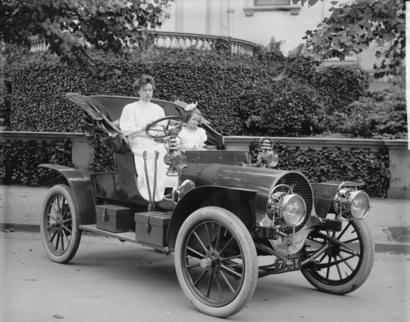
\includegraphics[width=\linewidth]{sample-franklin}
  \caption{1907 Franklin Model D roadster. Photograph by Harris \&
    Ewing, Inc. [Public domain], via Wikimedia
    Commons. (\url{https://goo.gl/VLCRBB}).}
  \Description{A woman and a girl in white dresses sit in an open car.}
\end{figure}

Your figures should contain a caption which describes the figure to
the reader.

Figure captions are placed {\itshape below} the figure.

Every figure should also have a figure description unless it is purely
decorative. These descriptions convey what’s in the image to someone
who cannot see it. They are also used by search engine crawlers for
indexing images, and when images cannot be loaded.

A figure description must be unformatted plain text less than 2000
characters long (including spaces).  {\bfseries Figure descriptions
  should not repeat the figure caption – their purpose is to capture
  important information that is not already provided in the caption or
  the main text of the paper.} For figures that convey important and
complex new information, a short text description may not be
adequate. More complex alternative descriptions can be placed in an
appendix and referenced in a short figure description. For example,
provide a data table capturing the information in a bar chart, or a
structured list representing a graph.  For additional information
regarding how best to write figure descriptions and why doing this is
so important, please see
\url{https://www.acm.org/publications/taps/describing-figures/}.

\subsection{The ``Teaser Figure''}

A ``teaser figure'' is an image, or set of images in one figure, that
are placed after all author and affiliation information, and before
the body of the article, spanning the page. If you wish to have such a
figure in your article, place the command immediately before the
\verb|\maketitle| command:
\begin{verbatim}
  \begin{teaserfigure}
    \includegraphics[width=\textwidth]{sampleteaser}
    \caption{figure caption}
    \Description{figure description}
  \end{teaserfigure}
\end{verbatim}

\section{Citations and Bibliographies}

The use of \BibTeX\ for the preparation and formatting of one's
references is strongly recommended. Authors' names should be complete
--- use full first names (``Donald E. Knuth'') not initials
(``D. E. Knuth'') --- and the salient identifying features of a
reference should be included: title, year, volume, number, pages,
article DOI, etc.

The bibliography is included in your source document with these two
commands, placed just before the \verb|\end{document}| command:
\begin{verbatim}
  \bibliographystyle{ACM-Reference-Format}
  \bibliography{bibfile}
\end{verbatim}
where ``\verb|bibfile|'' is the name, without the ``\verb|.bib|''
suffix, of the \BibTeX\ file.

Citations and references are numbered by default. A small number of
ACM publications have citations and references formatted in the
``author year'' style; for these exceptions, please include this
command in the {\bfseries preamble} (before the command
``\verb|\begin{document}|'') of your \LaTeX\ source:
\begin{verbatim}
  \citestyle{acmauthoryear}
\end{verbatim}


  Some examples.  A paginated journal article \cite{Abril07}, an
  enumerated journal article \cite{Cohen07}, a reference to an entire
  issue \cite{JCohen96}, a monograph (whole book) \cite{Kosiur01}, a
  monograph/whole book in a series (see 2a in spec. document)
  \cite{Harel79}, a divisible-book such as an anthology or compilation
  \cite{Editor00} followed by the same example, however we only output
  the series if the volume number is given \cite{Editor00a} (so
  Editor00a's series should NOT be present since it has no vol. no.),
  a chapter in a divisible book \cite{Spector90}, a chapter in a
  divisible book in a series \cite{Douglass98}, a multi-volume work as
  book \cite{Knuth97}, a couple of articles in a proceedings (of a
  conference, symposium, workshop for example) (paginated proceedings
  article) \cite{Andler79, Hagerup1993}, a proceedings article with
  all possible elements \cite{Smith10}, an example of an enumerated
  proceedings article \cite{VanGundy07}, an informally published work
  \cite{Harel78}, a couple of preprints \cite{Bornmann2019,
    AnzarootPBM14}, a doctoral dissertation \cite{Clarkson85}, a
  master's thesis: \cite{anisi03}, an online document / world wide web
  resource \cite{Thornburg01, Ablamowicz07, Poker06}, a video game
  (Case 1) \cite{Obama08} and (Case 2) \cite{Novak03} and \cite{Lee05}
  and (Case 3) a patent \cite{JoeScientist001}, work accepted for
  publication \cite{rous08}, 'YYYYb'-test for prolific author
  \cite{SaeediMEJ10} and \cite{SaeediJETC10}. Other cites might
  contain 'duplicate' DOI and URLs (some SIAM articles)
  \cite{Kirschmer:2010:AEI:1958016.1958018}. Boris / Barbara Beeton:
  multi-volume works as books \cite{MR781536} and \cite{MR781537}. A
  couple of citations with DOIs:
  \cite{2004:ITE:1009386.1010128,Kirschmer:2010:AEI:1958016.1958018}. Online
  citations: \cite{TUGInstmem, Thornburg01, CTANacmart}.
  Artifacts: \cite{R} and \cite{UMassCitations}.

\section{Acknowledgments}

The authors thank the instructors and peers of CMSC 725 for their feedback and support throughout the project. We also acknowledge the open data providers, including the US Census Bureau and regional transit agencies, whose datasets made this work possible. Special thanks to the developers of the open-source Python libraries used in this study, and to the broader research community for their foundational contributions to computational urbanism and network science.

\section{Conclusion}

This study demonstrates the power and flexibility of programmatic, data-driven approaches for the design and evaluation of urban rapid transit networks. By integrating geospatial analysis, graph algorithms, evolutionary optimization, and interactive visualization, we have developed a reproducible framework that generates alternative network designs tailored to the unique spatial and demographic characteristics of the Washington, DC metropolitan area. The results show that significant improvements in coverage, connectivity, and equity are achievable compared to the legacy WMATA Metro system, with only modest increases in network length and operational complexity. The use of open-source tools and transparent methodologies ensures that the process is both extensible and adaptable to other metropolitan regions. While several limitations remain—including the static nature of the demand model, the exclusion of certain socioeconomic variables, and the need for further stakeholder engagement—this work provides a robust foundation for future research and practical application. The framework's modularity supports ongoing refinement as new data, algorithms, and policy priorities emerge, and its emphasis on transparency and reproducibility aligns with best practices in computational urban science. Ultimately, this approach offers a promising path toward more equitable, efficient, and resilient urban mobility systems.

\section{References}

% The bibliography will be generated from sample-base.bib

% ...existing code...

\section{Appendices}

If your work needs an appendix, add it before the
``\verb|\end{document}|'' command at the conclusion of your source
document.

Start the appendix with the ``\verb|appendix|'' command:
\begin{verbatim}
  \appendix
\end{verbatim}
and note that in the appendix, sections are lettered, not
numbered. This document has two appendices, demonstrating the section
and subsection identification method.

\section{Multi-language papers}

Papers may be written in languages other than English or include
titles, subtitles, keywords and abstracts in different languages (as a
rule, a paper in a language other than English should include an
English title and an English abstract).  Use \verb|language=...| for
every language used in the paper.  The last language indicated is the
main language of the paper.  For example, a French paper with
additional titles and abstracts in English and German may start with
the following command
\begin{verbatim}
\documentclass[sigconf, language=english, language=german,
               language=french]{acmart}
\end{verbatim}

The title, subtitle, keywords and abstract will be typeset in the main
language of the paper.  The commands \verb|\translatedXXX|, \verb|XXX|
begin title, subtitle and keywords, can be used to set these elements
in the other languages.  The environment \verb|translatedabstract| is
used to set the translation of the abstract.  These commands and
environment have a mandatory first argument: the language of the
second argument.  See \verb|sample-sigconf-i13n.tex| file for examples
of their usage.

\section{SIGCHI Extended Abstracts}

The ``\verb|sigchi-a|'' template style (available only in \LaTeX\ and
not in Word) produces a landscape-orientation formatted article, with
a wide left margin. Three environments are available for use with the
``\verb|sigchi-a|'' template style, and produce formatted output in
the margin:
\begin{description}
\item[\texttt{sidebar}:]  Place formatted text in the margin.
\item[\texttt{marginfigure}:] Place a figure in the margin.
\item[\texttt{margintable}:] Place a table in the margin.
\end{description}

%%
%% The acknowledgments section is defined using the "acks" environment
%% (and NOT an unnumbered section). This ensures the proper
%% identification of the section in the article metadata, and the
%% consistent spelling of the heading.
\begin{acks}
To Robert, for the bagels and explaining CMYK and color spaces.
\end{acks}

%%
%% The next two lines define the bibliography style to be used, and
%% the bibliography file.
\bibliographystyle{ACM-Reference-Format}
\bibliography{sample-base}


%%
%% If your work has an appendix, this is the place to put it.
\appendix

\section{Research Methods}

\subsection{Part One}

Lorem ipsum dolor sit amet, consectetur adipiscing elit. Morbi
malesuada, quam in pulvinar varius, metus nunc fermentum urna, id
sollicitudin purus odio sit amet enim. Aliquam ullamcorper eu ipsum
vel mollis. Curabitur quis dictum nisl. Phasellus vel semper risus, et
lacinia dolor. Integer ultricies commodo sem nec semper.

\subsection{Part Two}

Etiam commodo feugiat nisl pulvinar pellentesque. Etiam auctor sodales
ligula, non varius nibh pulvinar semper. Suspendisse nec lectus non
ipsum convallis congue hendrerit vitae sapien. Donec at laoreet
eros. Vivamus non purus placerat, scelerisque diam eu, cursus
ante. Etiam aliquam tortor auctor efficitur mattis.

\section{Online Resources}

Nam id fermentum dui. Suspendisse sagittis tortor a nulla mollis, in
pulvinar ex pretium. Sed interdum orci quis metus euismod, et sagittis
enim maximus. Vestibulum gravida massa ut felis suscipit
congue. Quisque mattis elit a risus ultrices commodo venenatis eget
dui. Etiam sagittis eleifend elementum.

Nam interdum magna at lectus dignissim, ac dignissim lorem
rhoncus. Maecenas eu arcu ac neque placerat aliquam. Nunc pulvinar
massa et mattis lacinia.

\end{document}
\endinput
%%
%% End of file `sample-manuscript.tex'.
